\section{Results}
We discuss the results in three directions, hedging effectiveness,
ability of hedging extreme negative events in $R^S$, and the stability of $h^*$.

\subsection{Hedging Effectiveness}
The hedging effectiveness(HE) is defined as
\begin{align}
  1- \frac{\rho_\phi(R^h)}{\rho_\phi(R^S)}.
  \end{align}
The hedging effectiveness is the reduction of portfolio risk.
This way of evaluating of hedging performance is proposed by Ederington (1979) in the context of ...
He evaluates the extent of variance reduction by introducing another asset.
We measure the hedging effectiveness also in other risk measure mentioned in section \ref{subsec:spectral-risk-measures},
for example
\begin{align}
  1- \frac{\text{ES}_\alpha(R^h)}{\text{ES}_\alpha(R^S)}.
  \end{align}

Figure \ref{fig:OOSHE} shows the out-of-sample hedging effectiveness of difference copulas under various risk
reduction objectives.
Observe that in every copulas perform well in most of the time.
The average HE of copulas and risk reduction objectives is higher than 60\% except for Frank-copula.
However, the HEs vary a lot in every copula.
In some instances, the HE can be as low as 10\%.


%\begin{figure}[t]
%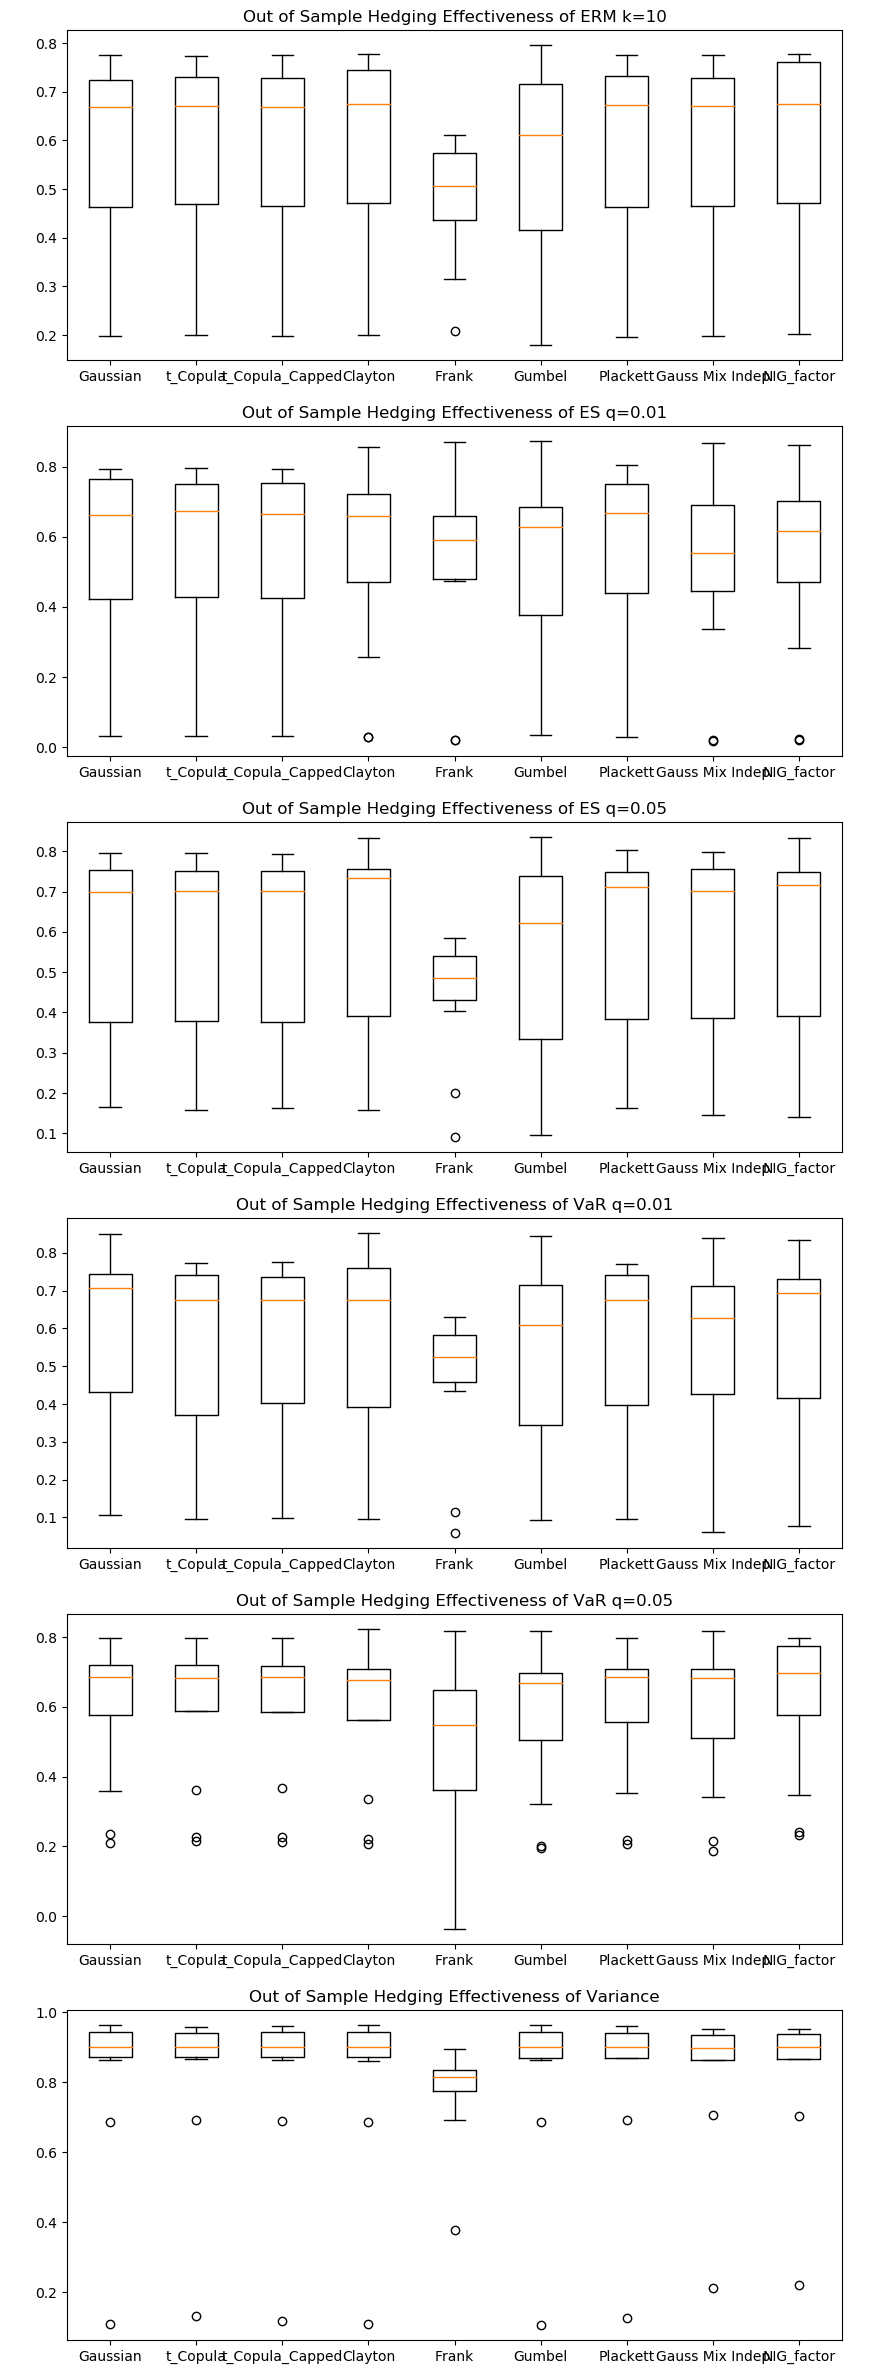
\includegraphics[width=\textwidth, height=\textheight]{_pics/Out of Sample Hedging Effectiveness.png}
%  \caption{}
%\label{out of Sample Hedging Effectieness}
%\end{figure}

\begin{figure}[!th]
   \centering
   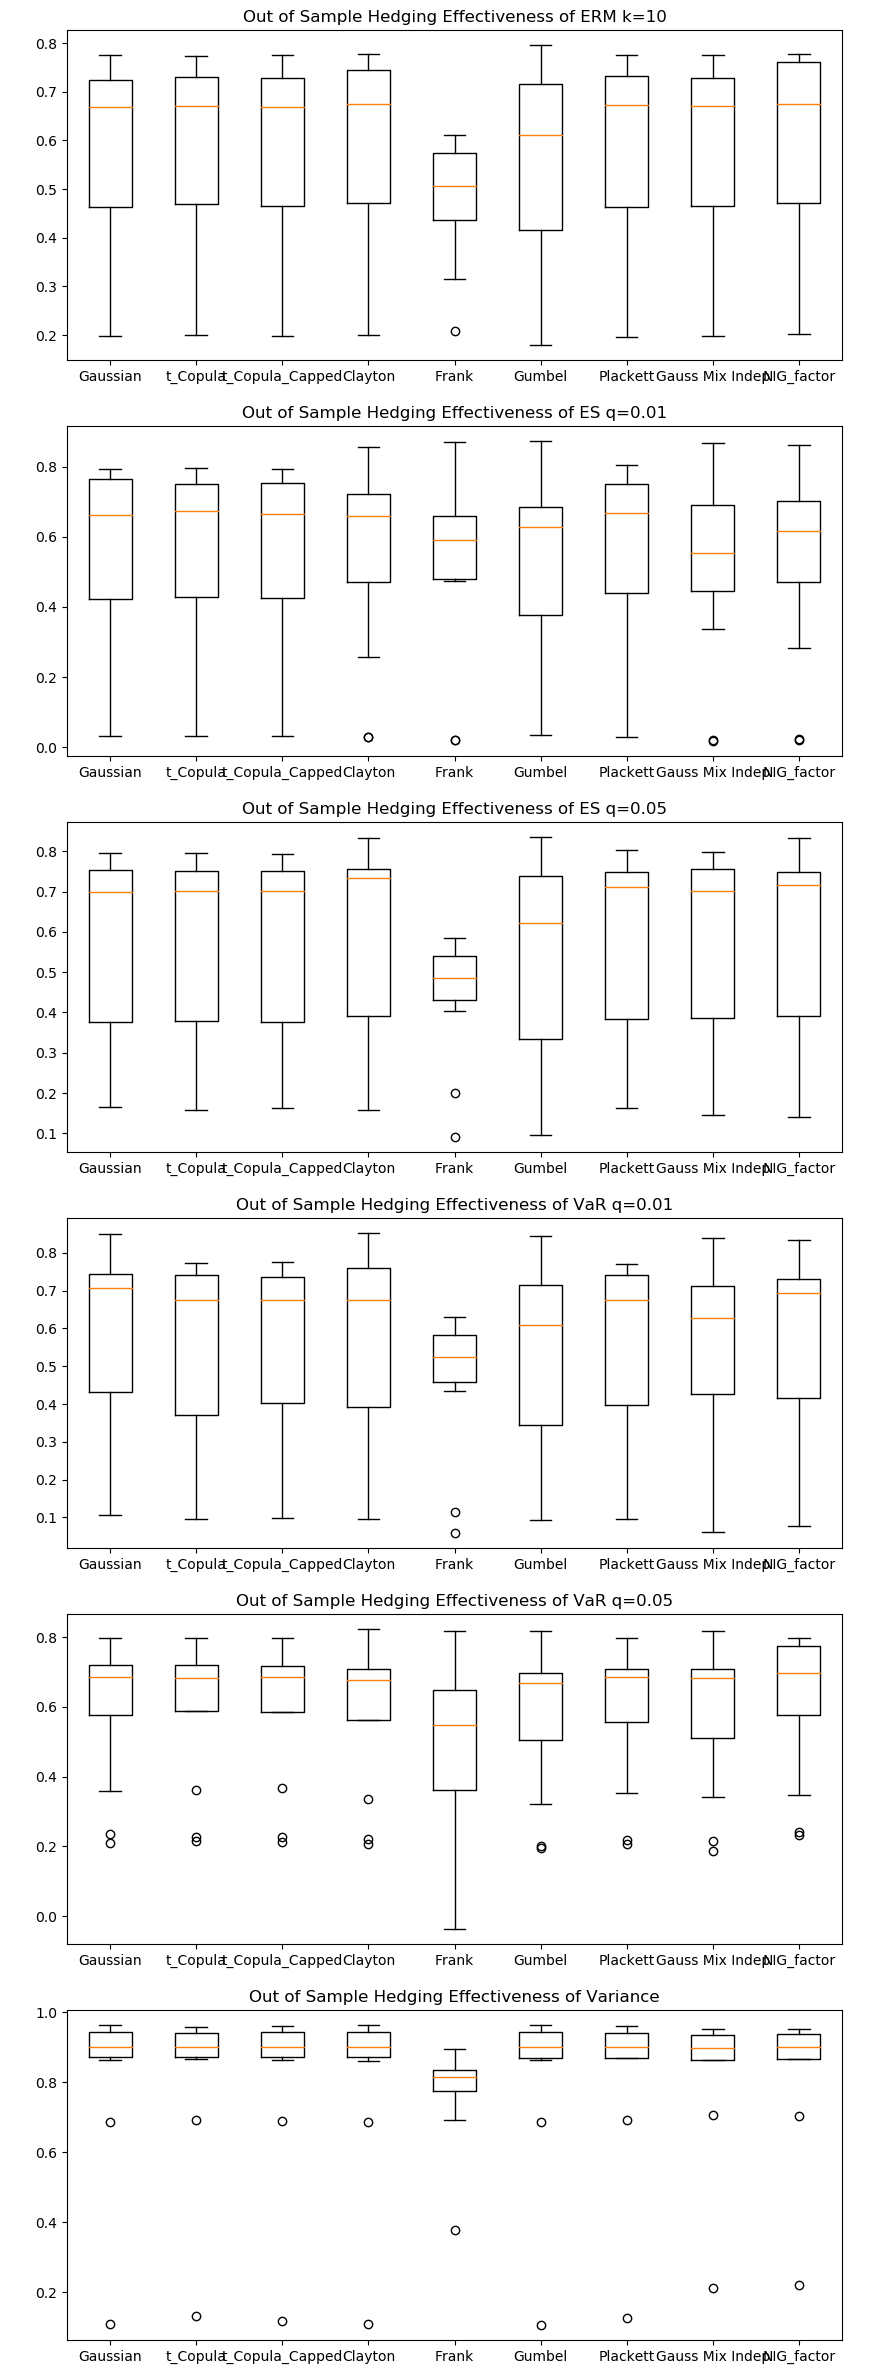
\includegraphics[height=25cm]{_pics/Out of Sample Hedging Effectiveness.png}
   \caption{Out of Sample Hedging Effectiveness Boxplot.
   The HEs are obtained from a set of out-of-sample data,
   each set consists 30 days log returns of Bitcoin and CME future.
   }
   \label{fig:OOSHE}
\end{figure}

\subsection{Ability of hedging extreme negative events}
Figure~\ref{fig:Gumbel} shows the time series of out-of-sample $R^h$ using Gumbel copula with the
objective of reducing variance.
The red dots are the 30 most extreme negative returns in Bitcoin.
In the figure, we can see the downside risk of Bitcoin is well managed by the hedging procedure with Gumbel copula.
Most of the extreme losses of Bitcoin are greatly reduced by introducing the CME future in the hedged portfolio.
Two exceptions are found in 25/09/2019 and 26/09/2019, where the CME future failed to follow the large drop in Bitcoin. (TODO: drop reason)
One of the possible reason is that traders was performing rollover activities on 25-26/09/2019, which
27/09/2019 is the expiry day of the September future.
Another reason for Gumbel fail of capturing the loss is dependence break.
The Kendall's tau in the training data is 0.2 higher than that of the testing data.
Other copulas suffer from the break as well.

\begin{figure}[!th]
   \centering
   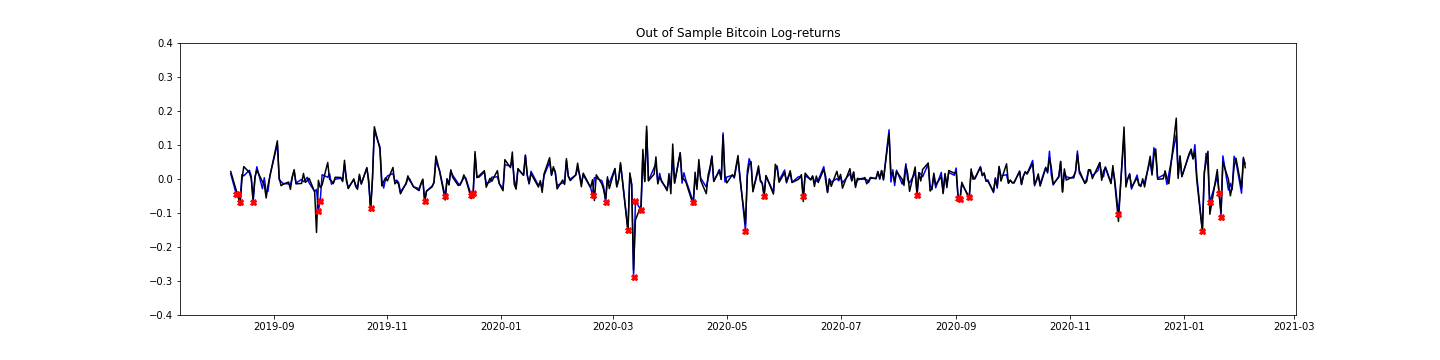
\includegraphics[width=\textwidth]{_pics/OOSBitcoin.png}
   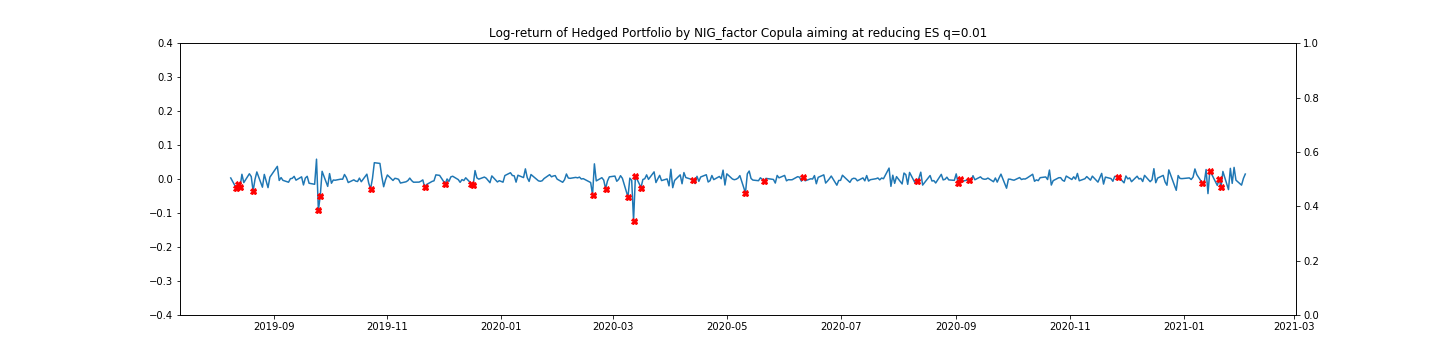
\includegraphics[width=\textwidth]{_pics/Gumbel_rh.png}
   \caption{Upper Panel: Out of Sample Log-return of Bitcoin; Lower Panel: Out of Sample Hedged Portfolio log-returns.
   The $h^*$ is obtained from Gumbel copula aiming at reducing variance.
   The red dots indicate the 30 most extreme negative returns in Bitcoin.
   }
   \label{fig:Gumbel}
\end{figure}

\subsection{Stability of $h^*$}
We measure the stability of $h^*$ by sum of absolute change
\begin{align}
    \sum_{t=1}^T|h_t - h_{t-1}|.
    \end{align}

Adjustment of portfolio weights induces price slippage (ref) and transaction cost.
From figure \ref{SAD} we know the NIG factor copula with variance as risk reduction objective generates the smallest
sum of absolute change in OHR.

\begin{figure}[!th]
   \centering
   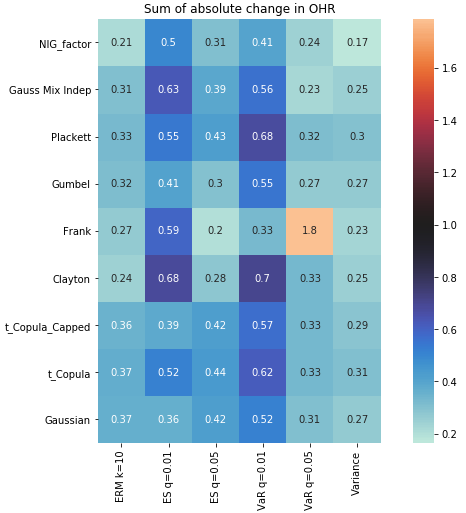
\includegraphics[width=\textwidth]{_pics/Sum of absolute change in OHR.png}
   \caption{Sum of Absolute Change in OHR.
   }
   \label{fig:SAD}
\end{figure}